% ===================================================================
\section{Conduction and thermal networks}\label{sec:conduction}
% ===================================================================
\begin{multicols}{2}
\subsection{Fourier's law; flux vs rate}\label{sec:fourier}
\CORE{}
\begin{formulabox}
\vspace{-6pt}
\begin{align}
\mathbf{q}'' &= -k\,\nabla T,\qquad q''_x=-k\frac{\dd T}{\dd x} \label{F:transfer:fourier}\\
\dot Q &= q''A = \frac{kA\,(T_1-T_2)}{L}\ \ (\text{plane wall, steady}) \label{F:transfer:wall}
\end{align}
\end{formulabox}
$q''$ = heat \textbf{flux} (\si{W/m^2}); $\dot Q$ = heat \textbf{rate} (\si{W}); $k$ in \si{W/(m.K)}. Heat flows down the temperature gradient (minus sign). Plane wall with constant $k$ and no generation: linear $T(x)$; a lower-$k$ layer carries a \emph{steeper} gradient for the same flux.

\subsection{Resistances and networks}\label{sec:resistances}
\CORE{} Steady, one-dimensional, no generation: $\dot Q=\Delta T/R_{\text{tot}}$.
\begin{formulabox}
\vspace{-6pt}
\begin{align}
R_{\text{wall}} &= \frac{L}{kA},\qquad R_{\text{conv}}=\frac{1}{hA},\qquad R_{\text{rad}}=\frac{1}{h_rA} \label{F:transfer:Rwall}\\
R_{\text{cyl}} &= \frac{\ln(r_2/r_1)}{2\pi kL} \label{F:transfer:Rcyl}\\
R_{\text{sph}} &= \frac{1}{4\pi k}\Big(\frac{1}{r_1}-\frac{1}{r_2}\Big) \label{F:transfer:Rsph}\\
R_{\text{contact}} &= R''_{tc}/A \label{F:transfer:Rcontact}\\
\text{series: } R &= \textstyle\sum R_i;\qquad \text{parallel: } \frac1R=\sum\frac{1}{R_i} \label{F:transfer:network}\\
\dot Q &= UA\,\Delta T_{\text{overall}},\qquad UA=1/R_{\text{tot}} \label{F:transfer:U}
\end{align}
\end{formulabox}
\textbf{Area basis of $U$.} For a cylinder, $U_iA_i=U_oA_o=1/R_{\text{tot}}$ but $U_i\ne U_o$; always state which area. Convection and radiation from one surface act in \emph{parallel} (same $\Delta T$ if surroundings $\approx$ fluid temperature).

\begin{reffig}{fig:network}{Composite wall: films and layers in series; a stud forms a parallel (bridging) path. Each box is a resistance.}
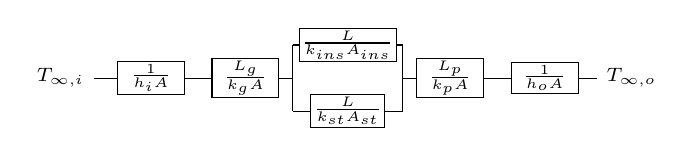
\begin{tikzpicture}[font=\scriptsize,res/.style={draw,minimum width=0.85cm,minimum height=0.36cm,inner sep=1pt}]
 \node (Ti) at (0,0) {$T_{\infty,i}$};
 \node[res] (a) at (1.15,0) {$\frac{1}{h_iA}$};
 \node[res] (b) at (2.35,0) {$\frac{L_g}{k_gA}$};
 \node[res] (c1) at (3.65,0.42) {$\frac{L}{k_{\text{ins}}A_{\text{ins}}}$};
 \node[res] (c2) at (3.65,-0.42) {$\frac{L}{k_{\text{st}}A_{\text{st}}}$};
 \node[res] (d) at (4.95,0) {$\frac{L_p}{k_pA}$};
 \node[res] (e) at (6.15,0) {$\frac{1}{h_oA}$};
 \node (To) at (7.25,0) {$T_{\infty,o}$};
 \draw (Ti)--(a)--(b)--(2.95,0); \draw (2.95,0.42)--(2.95,-0.42);
 \draw (2.95,0.42)--(c1)--(4.35,0.42); \draw (2.95,-0.42)--(c2)--(4.35,-0.42);
 \draw (4.35,0.42)--(4.35,-0.42); \draw (4.35,0)--(d)--(e)--(To);
\end{tikzpicture}
\end{reffig}

\textbf{Parallel-path assumption.} Treating stud and cavity as separate 1D paths assumes no sideways heat flow between them; the real 2D answer lies between this ``parallel-path'' result and an ``isothermal-planes'' estimate.\src{EK} \textbf{Thermal bridges} (studs, screws, metal frames, a beaker's support) are low-$R$ paths that short-circuit insulation.

\textbf{Contact resistance} arises from microscopic gaps at an interface; it falls with clamping pressure, soft interface materials, or thermal paste.

\subsection{R-values (insulation ratings)}\label{sec:rvalue}
\CORE{} Per-unit-area resistance $R''=L/k$ (\si{m^2.K/W}) is the SI ``RSI''. US $R$-value uses \si{ft^2.\degF.h/Btu}.
\begin{formulabox}
\begin{equation}
R_{\text{US}} = 5.678\,R_{\text{SI}},\qquad R_{\text{SI}}=0.1761\,R_{\text{US}} \label{F:transfer:rvalue}
\end{equation}
\end{formulabox}
($1\ \si{ft^2.\degF.h/Btu}=\SI{0.176110}{m^2.K/W}$, IT Btu.)\src{PINT} R-values of layers in series add; $U''=1/R''_{\text{total}}$ including surface films. Parallel paths combine through $U$ (area-weighted), \emph{not} by averaging $R$.

\begin{demobox}\anchor{demo:wall}\textbf{Composite wall with studs.} Per \si{m^2}: inside film $h_i=8$, outside $h_o=\SI{25}{W/(m^2.K)}$ (given); gypsum \SI{12.7}{mm} ($k=0.16$); \SI{89}{mm} cavity of mineral wool ($k=0.040$) or pine stud ($k=0.092$); plywood \SI{12}{mm} ($k=0.0907$).
Resistances (\si{m^2.K/W}): films $0.125+0.040$; gypsum 0.079; plywood 0.132; wool 2.225; stud 0.967.
Cavity path $R''=2.602$ (US R-14.8); stud path 1.344. With \SI{15}{\percent} studs: $U''=0.85/2.602+0.15/1.344=\SI{0.438}{W/(m^2.K)}$, so whole-wall $R''=2.28$ (US R-13.0): bridging costs \SI{12}{\percent}. At $\Delta T=\SI{20}{K}$: $q''=\SI{8.8}{W/m^2}$.
\emph{Check:} conversion factor confirmed with a unit library; $R_{\text{stud}}<R_{\text{eff}}<R_{\text{cav}}$ \checkmark.\src{MAT}\src{PINT}\end{demobox}

\subsection{Critical radius of insulation}\label{sec:critradius}
Adding insulation to a \emph{small} cylinder or sphere increases outer area (lower convection resistance) while adding conduction resistance. Heat loss is maximal at
\begin{equation}
r_{\text{cr,cyl}}=\frac{k_{\text{ins}}}{h},\qquad r_{\text{cr,sph}}=\frac{2k_{\text{ins}}}{h}. \label{F:transfer:rcrit}
\end{equation}
If the bare radius is below $r_{\text{cr}}$, thin insulation \emph{increases} loss (e.g.\ $k=0.04$, $h=10$: $r_{\text{cr}}=\SI{4}{mm}$---relevant for wires, not for a beaker).\src{DER}

\begin{demobox}\anchor{demo:container}\textbf{Where does an insulated container lose heat?} (Idealized geometry for illustration; not a design or rule-verified device.) Water at \SI{60}{\celsius}, \SI{0.400}{kg}, in a thin can of radius \SI{4.0}{cm}, height \SI{12}{cm}, wrapped radially in EPS ($k=\SI{0.0355}{W/(m.K)}$, \tref{T:conductivity}) to radius \SI{6.0}{cm}; \SI{2.0}{cm} EPS discs top and bottom; still air at \SI{22}{\celsius}; outer $\varepsilon=0.90$; water-side film neglected.
Side: $R_{\text{ins}}=\ln(6/4)/(2\pi\cdot0.0355\cdot0.12)=\SI{15.15}{K/W}$. Solving the outer-surface balance gives $T_o=\SI{27.4}{\celsius}$, $h_c=3.5$ (C6), $h_r=\SI{5.4}{W/(m^2.K)}$, $R_{\text{out}}=\SI{2.48}{K/W}$ (insulation is \SI{86}{\percent} of the side resistance). Each disc: $R\approx\SI{122}{K/W}$.
Total $K=1/17.63+2/122=\SI{0.073}{W/K}$; $C=\SI{1672}{J/K}$; $\tau=C/K=\SI{6.3}{h}$; after \SI{30}{min}: \SI{57.1}{\celsius}.
\emph{Lessons:} with good insulation the outer finish barely matters; seams, lids, and supports (bridges) usually dominate real losses, and an open top adds evaporation (\pg{sec:boiling}). Curvature check for C6 fails slightly here too, so $h_c$ is a mild underestimate.\src{DER}\src{HT}\src{CP}\end{demobox}

\subsection{Diffusivity, the heat equation, boundary conditions}\label{sec:heateq}
\begin{formulabox}
\vspace{-6pt}
\begin{align}
\alpha &= \frac{k}{\rho c_p}\ \ (\si{m^2/s}) \label{F:transfer:diffusivity}\\
\frac{\partial T}{\partial t} &= \alpha\,\frac{\partial^2T}{\partial x^2}+\frac{\dot q}{\rho c_p}\ \ (\text{1D, const.\ } k) \label{F:transfer:heateq}
\end{align}
\end{formulabox}
High $\alpha$ = temperature changes propagate quickly (metals); $k$ alone sets steady flux. Penetration depth after time $t$ scales as $\sqrt{\alpha t}$.

\begin{reftab}{T:bcs}{Boundary conditions at a surface $x=0$.\src{EK}}
\small
\begin{tabularx}{\linewidth}{@{}L{0.30\linewidth}Y@{}}
\toprule
Type & Condition\\
\midrule
Specified temperature & $T(0,t)=T_s$\\
Specified flux & $-k\,\partial T/\partial x|_0=q''_s$\\
Insulated / symmetry & $\partial T/\partial x|_0=0$\\
Convection & $-k\,\partial T/\partial x|_0=h\,[T(0,t)-T_\infty]$\\
Perfect-contact interface & $T$ and $q''$ continuous\\
\bottomrule
\end{tabularx}\end{reftab}

\EXT{} \textbf{Uniform generation} $\dot q$ (\si{W/m^3}), surfaces at $T_s$: plane wall of thickness $2L$: $T_{\max}=T_s+\dot qL^2/(2k)$; long cylinder of radius $r_0$: $T_{\max}=T_s+\dot q r_0^2/(4k)$. \textbf{Fins} help most where $h$ is small (gases) and fin $k$ is large; an infinitely long fin transfers $\sqrt{hPkA_c}\,(T_b-T_\infty)$.\src{EK}
\end{multicols}

\begin{reftab}{T:conductivity}{Thermal conductivity $k$, density $\rho$, and specific heat $c_p$ near room temperature. Building/insulation entries are \emph{design values} for typical grades (not pure-element values); real products vary with density, moisture, and age.\src{MAT} Source codes: EN12524 = DIN EN 12524:2000; ASHRAE = Handbook Fundamentals 2013; air row from the Lemmon--Jacobsen model.\src{CP}}
\small
\begin{tabularx}{\textwidth}{@{}Yrrrl@{}}
\toprule
Material & $k$ (\si{W/(m.K)}) & $\rho$ (\si{kg/m^3}) & $c_p$ (\si{J/(kg.K)}) & Source\\
\midrule
\tabinput{data/conductivity.tex}
\bottomrule
\end{tabularx}\end{reftab}
